\newif\ifinria
\def\ptitle{Recoloring graphs with Kempe changes} % Title
\def\pauthor{Clément Legrand-Duchesne} % Author
\def\padvisors{Marthe Bonamy, Vincent Delecroix} % Advisors
\def\pteam{Graphe et Optimisation, Combinatoire et Interactions} % Team
\def\pinstitute{Univ. Bordeaux, LaBRI, France} % Affiliation
\def\pdate{Thursday April 6, 2023} % Date
\inriatrue % inriatrue/inriafalse to enable/disable Inria logo

\pdfobjcompresslevel=0
\documentclass[final,hyperref={pdfpagelabels=false},xcolor=dvipsnames]{beamer}
\usepackage[orientation=portrait,size=a0,scale=1.4]{beamerposter}
\usepackage[utf8]{inputenc}
\usepackage[sfdefault]{roboto}
\usepackage[english]{babel}
\usepackage{amsmath, amsthm, amssymb, array, booktabs, grffile, latexsym, tabularx, xspace}
\newcolumntype{Z}{>{\centering\arraybackslash}X}
\newcommand{\pphantom}{\textcolor{ta3aluminium}}
\newlength{\columnheight}

\def\plogo{logo/logo_LaBRI.png}
\def\purl{https://www.labri.fr/}
\def\pmail{Twitter: @labriOfficial}

\mode<presentation>{\usetheme{SDSLaBRI}}
\title[\ptitle]{\texorpdfstring{\huge \ptitle}{\ptitle}}
\author[\pauthor]{\pauthor\ -\ \padvisors}
\institute[\pinstitute]{\pteam\ -\ \pinstitute}
\date[\pdate]{\pdate}
\setlogo{\plogo}
\setauthorurl{\purl}
\setauthoremail{\pmail}


\graphicspath{{./fig/}} % Figures and logos directory
\setlength{\columnheight}{588ex} % Tweak this value if columns are too long/short (should be okay with 588ex)

\begin{document}
\begin{frame}
  \begin{columns}
    \begin{column}{.49\textwidth}
      \begin{beamercolorbox}[center,wd=\textwidth]{postercolumn}
        \begin{minipage}[T]{.95\textwidth}
          \parbox[t][\columnheight]{\textwidth}{
            
            \begin{block}{Video content consumption}
            
            \centering
            
            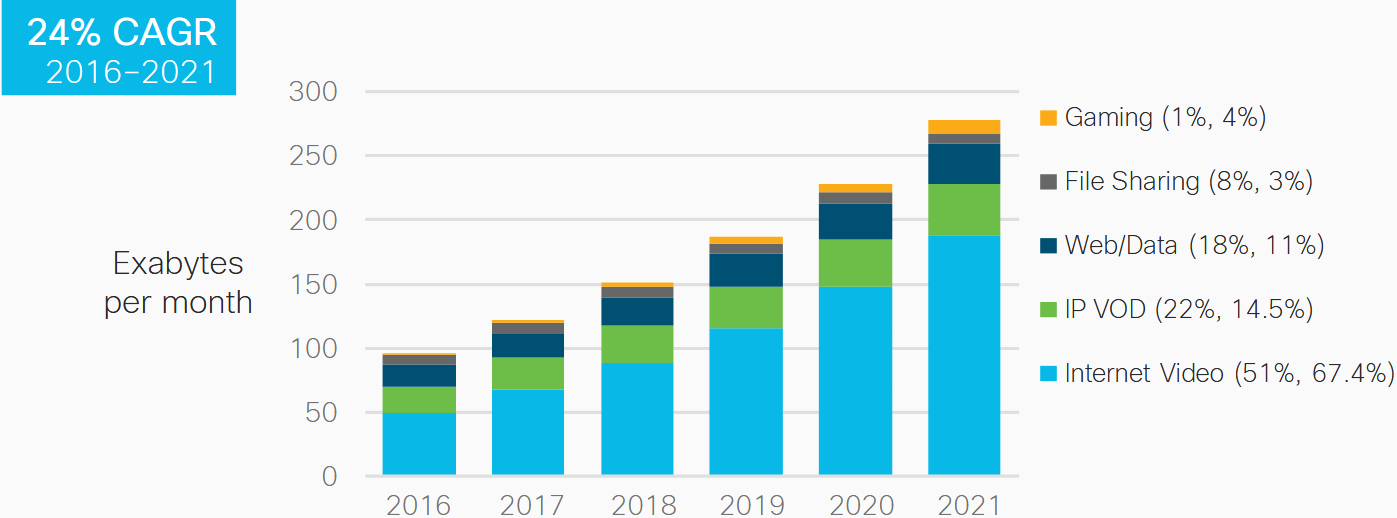
\includegraphics[width=.925\textwidth]{sample/cisco-vni-2021.png}            
            
            \end{block}
            
            \vfill
            
            \begin{block}{Content Delivery Networks (CDN)}
            
            \centering
            
            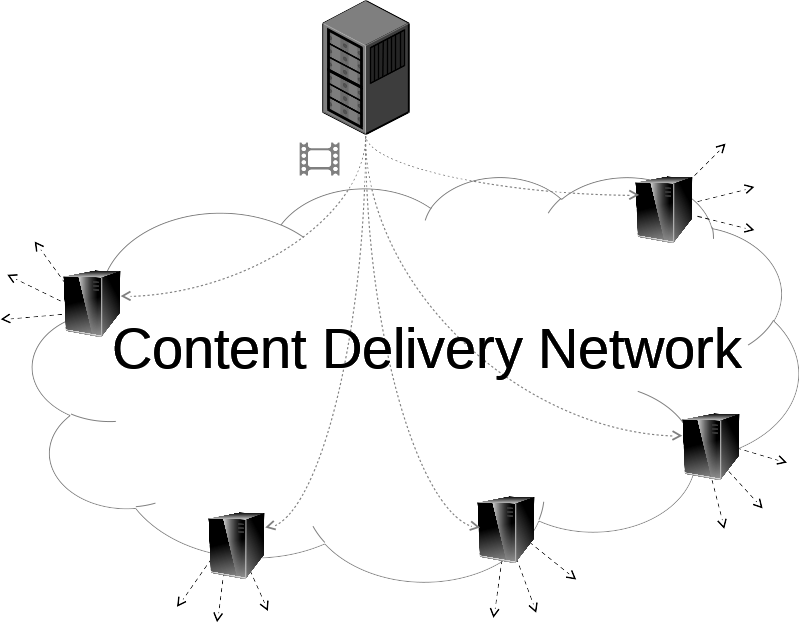
\includegraphics[width=.33\textwidth]{sample/CDN.png}
            
            \end{block}
            
            \vfill
            
            \begin{block}{HTTP Adaptive Streaming (HAS)}
            
            \centering
            
            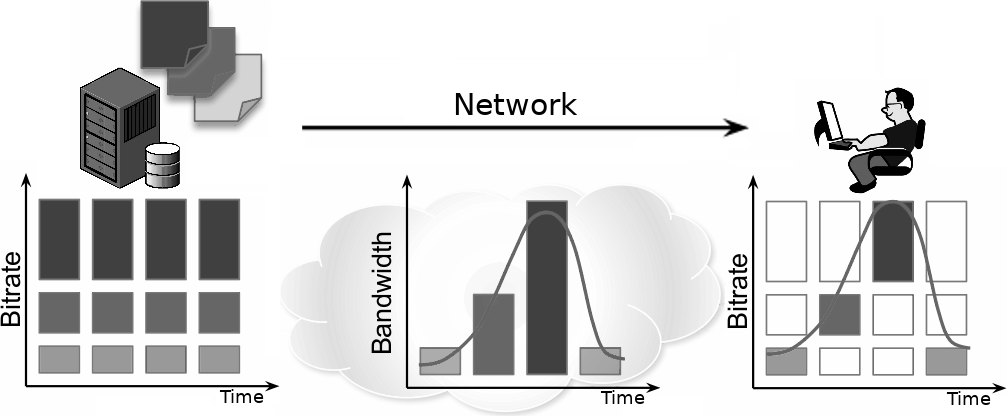
\includegraphics[width=.925\textwidth]{sample/DASH-2.png}
            
            \end{block}
            
            \vfill
            
            \begin{block}{MS-Stream: Multi-Source Streaming over HTTP}
            
            \centering
            
            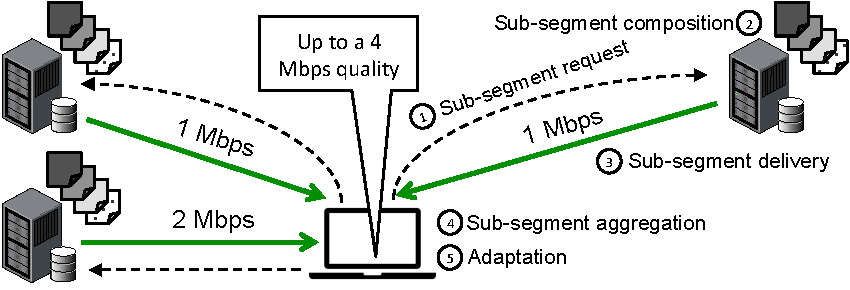
\includegraphics[width=.925\textwidth]{sample/msstream_archi.pdf}
            
            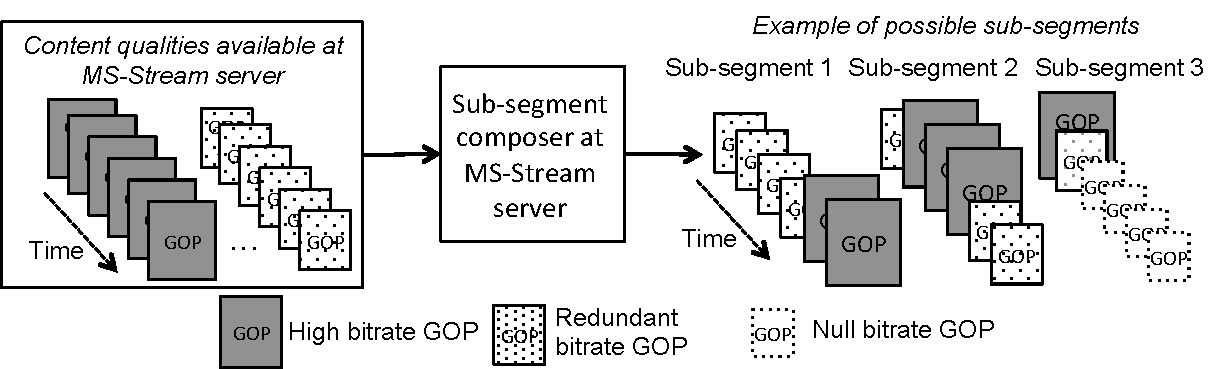
\includegraphics[width=.925\textwidth]{sample/chunk2.pdf}
            
            \end{block}
            
            \vfill
            
            \begin{block}{Problem statement}
            
            \centering
            
            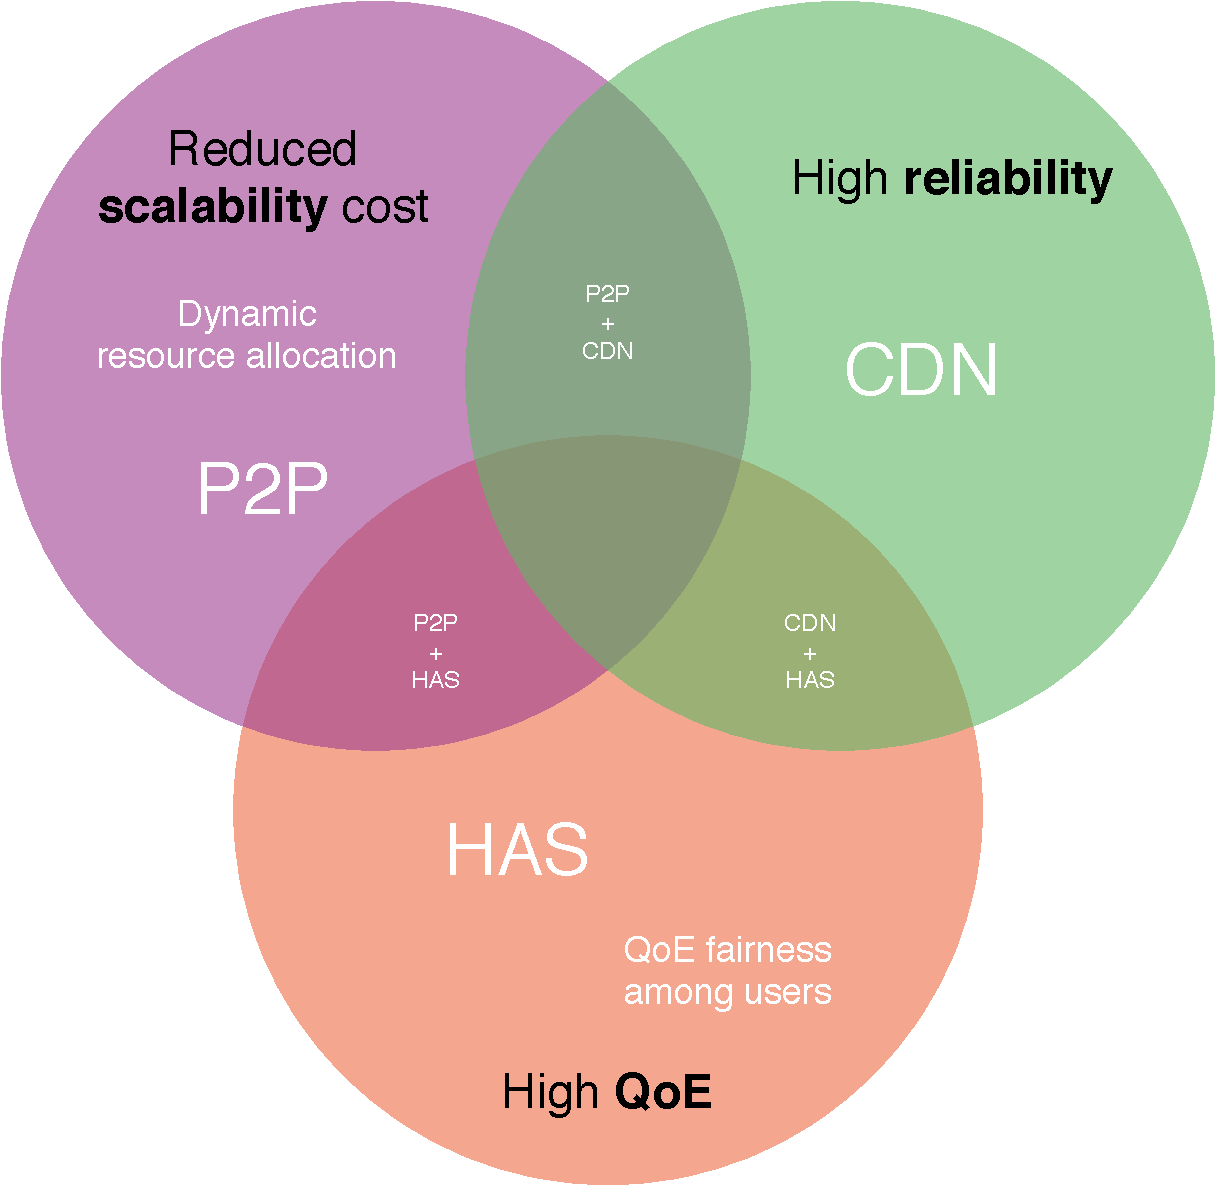
\includegraphics[width=.5\textwidth]{sample/SotA-cropped.pdf}
            
            \end{block}
            
          }
        \end{minipage}
      \end{beamercolorbox}
    \end{column}
    \begin{column}{.49\textwidth}
      \begin{beamercolorbox}[center,wd=\textwidth]{postercolumn}
        \begin{minipage}[T]{.95\textwidth}
          \parbox[t][\columnheight]{\textwidth}{
            
            \begin{block}{ idea}
            
            \begin{itemize}
            
            \item Reliability, QoE and scalability
            
            MS-Stream: Multiple-Source adaptive streaming over HTTP
            
            \item Incentive to contribute
            
            Rewarding: contributing users get a higher quality
            
            \item End-users privacy
            
            TEE (SGX): encryption, NAT and anonymity
            
            \end{itemize}
            
            \end{block}
            
            \vfill
            
            \begin{block}{ overview}
            
            \centering
            
            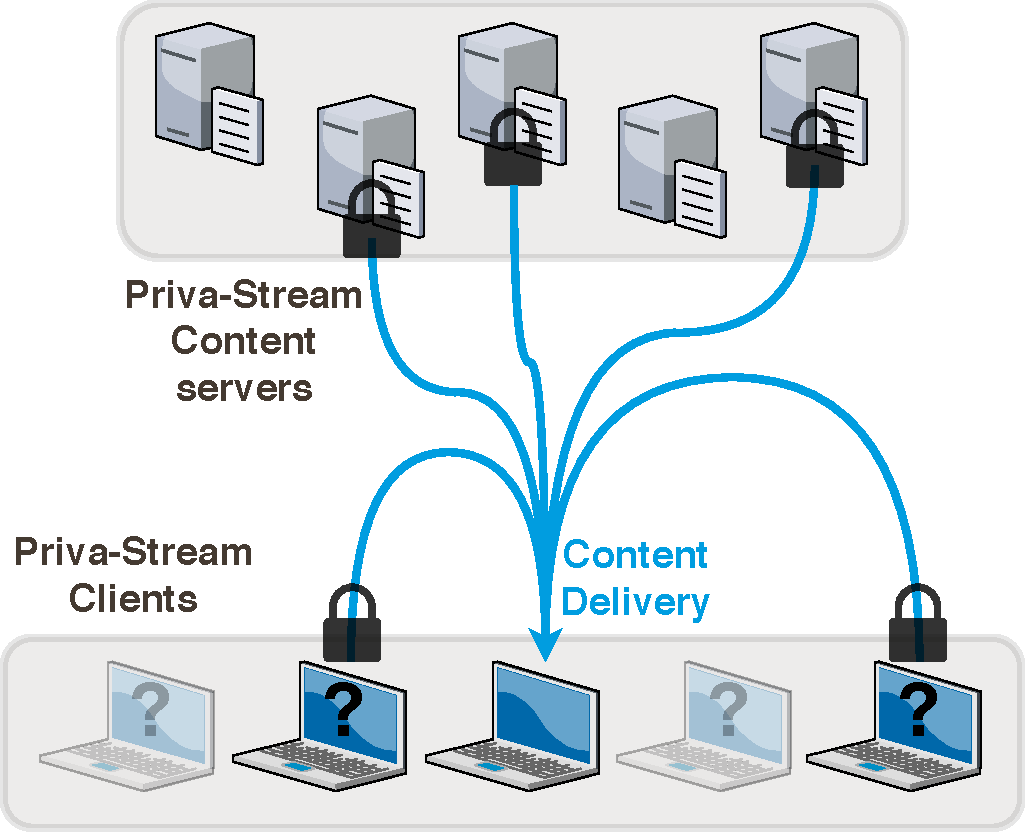
\includegraphics[width=.925\textwidth]{sample/BP.pdf}
            
            \end{block}
            
            \vfill
            
            \begin{block}{ technical description}
            
            \centering
            
            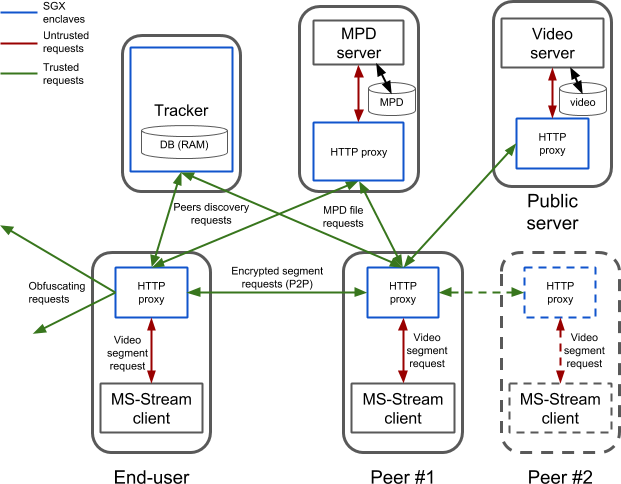
\includegraphics[width=.8\textwidth]{sample/PS-tech.png}
            
            \end{block}
            
            \vfill
            
            \begin{block}{ early results}
            
            \centering
            
            Experiment: Four clients joining the system sequentially
            
            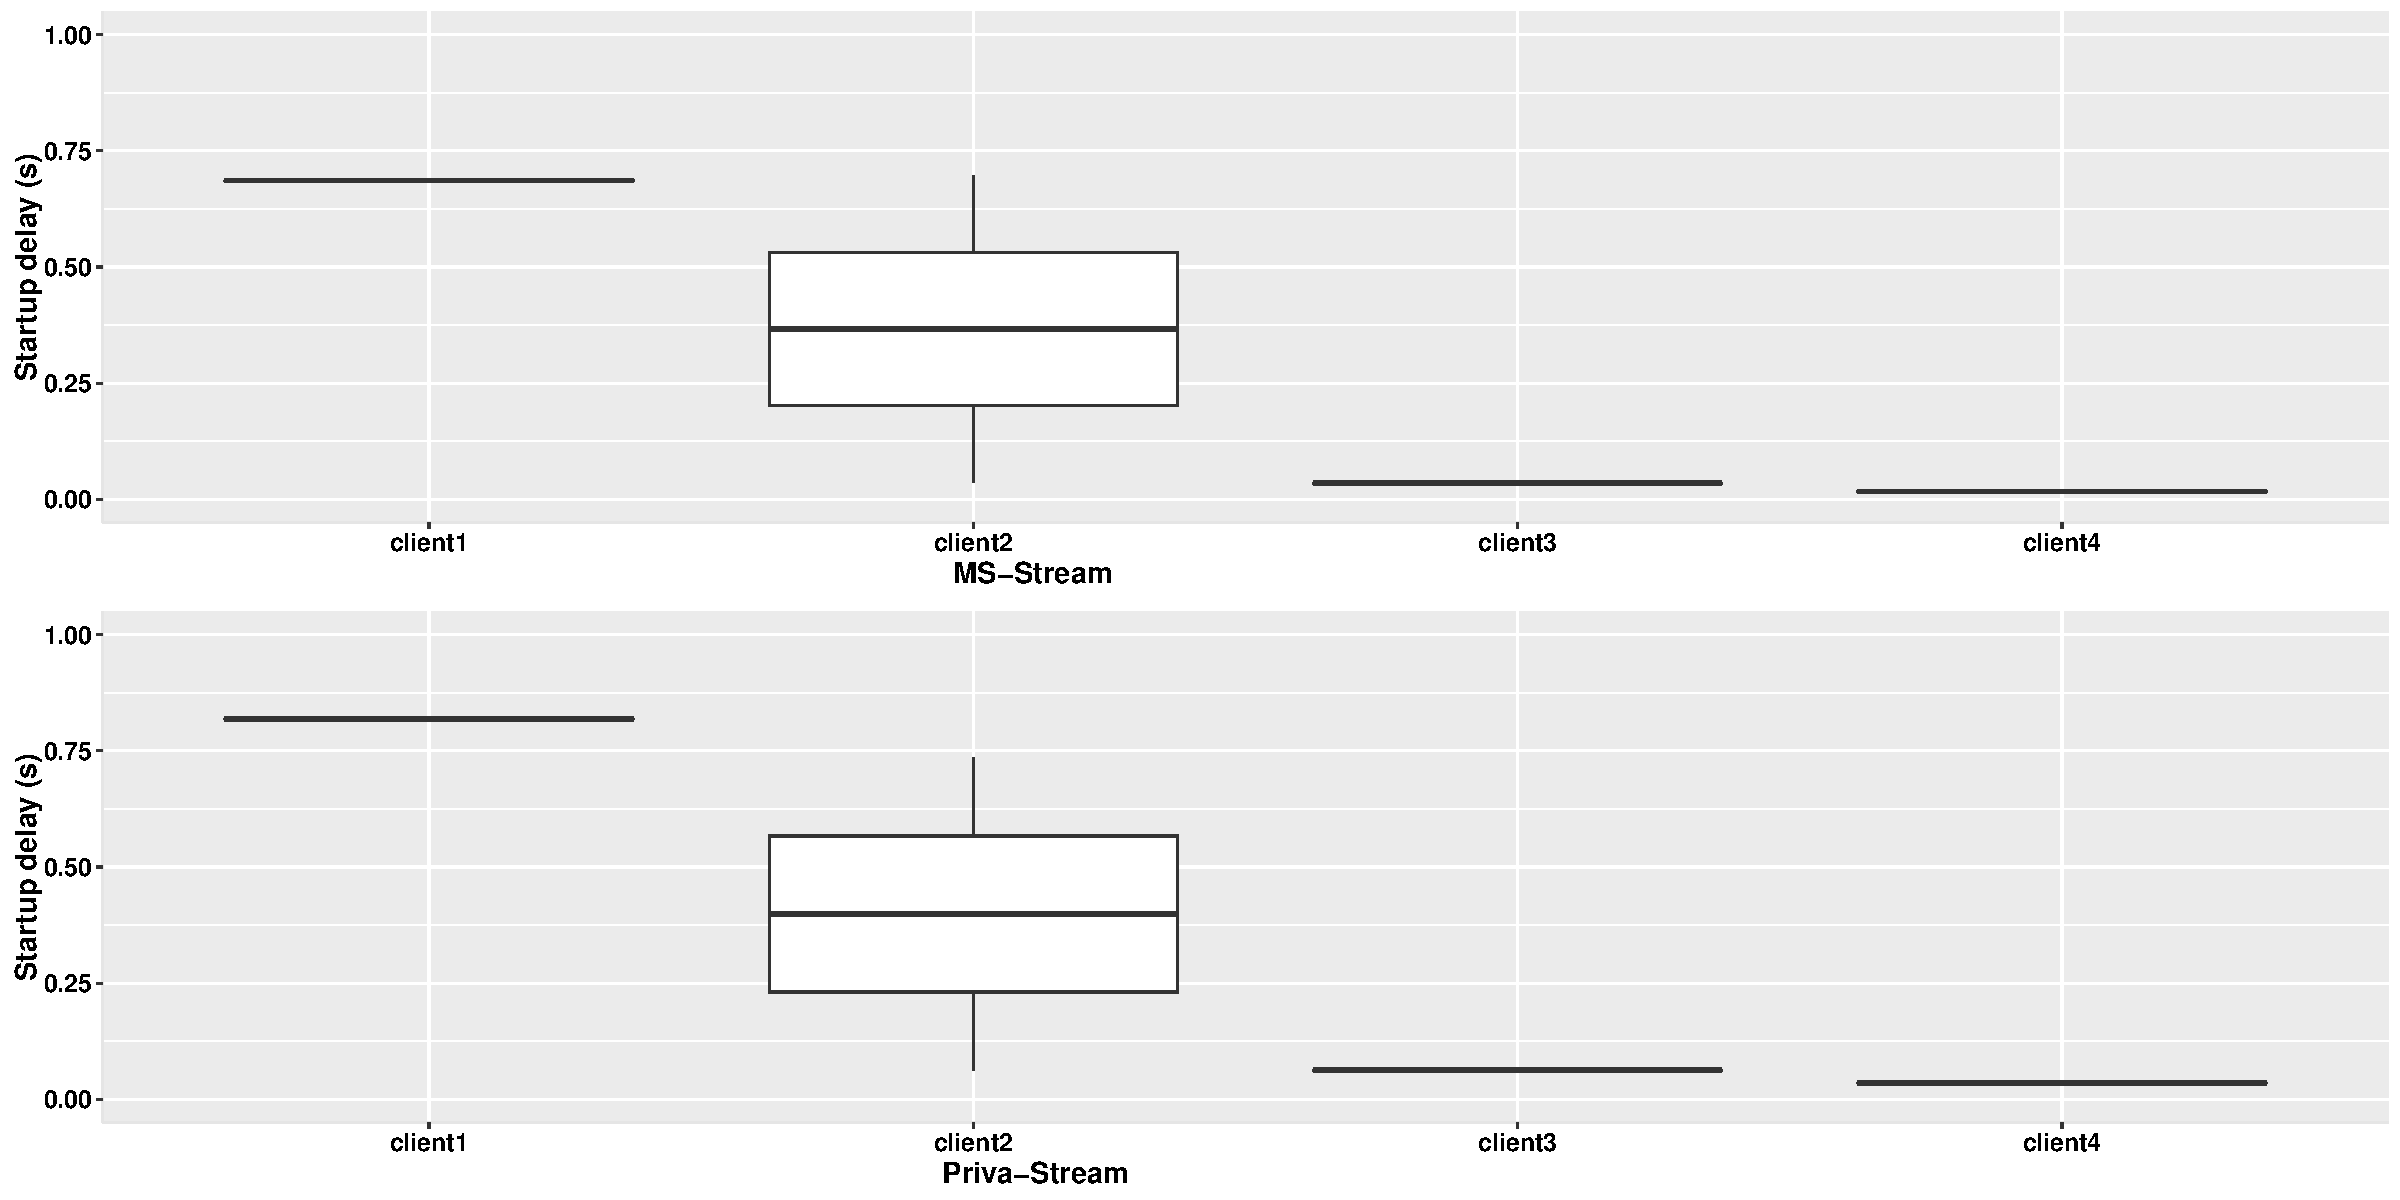
\includegraphics[width=.925\textwidth]{sample/startup.pdf}
            
            Startup delay (s) - MS-Stream (top) vs (bottom)
            
            \end{block}
            
          }
        \end{minipage}
      \end{beamercolorbox}
    \end{column}
  \end{columns}
  \vskip1ex
\end{frame}
\end{document}
